


\begin{frame}{LIVE DEMO}
  \vspace*{2cm}
   \begin{center} \Large \textbf{LIVE DEMO} \\ \normalsize Let's enhance PETSc together!\end{center}
  \begin{flushright} \vspace*{3cm}
   \begin{flushright}
   \textit{Debugging does not mean just trying a bunch of random things \\
           with no understanding and hoping to figure out the problem.}
  \end{flushright}
  \end{flushright}
\end{frame}


\begin{frame}[fragile]{In a Nutshell}

 \begin{block}{Create Pull Request in BitBucket}
  \begin{itemize}
   \item Fork the repository at \verb|https://bitbucket.org/petsc/petsc/|
   \item Create a new branch off master: \verb|git checkout -b myname/mybranchname|
   \item Apply changes
   \item Commit changes: \verb|git commit -a|
   \item Push changes: \verb|git push -u origin myname/mybranchname|
   \item Create pull request to master branch in main PETSc repository via webinterface
  \end{itemize}
 \end{block}
 
 \begin{block}{Prefer GitHub?}
  \begin{itemize}
   \item You may also fork our mirror at GitHub
   \item Repeat steps above
  \end{itemize}
 \end{block}
 
\end{frame}



%
% Git branches
%
\section{PETSc and Git}

\begin{frame}{PETSc}
   \begin{center} \Large \textbf{What about all those branches in the repository?} \end{center}
  \begin{flushright} \vspace*{4cm}
   \textit{git sucks!}
  \end{flushright}
\end{frame}



\begin{frame}{PETSc and Git}
  \begin{block}{PETSc's Workflow}
  \begin{center}
    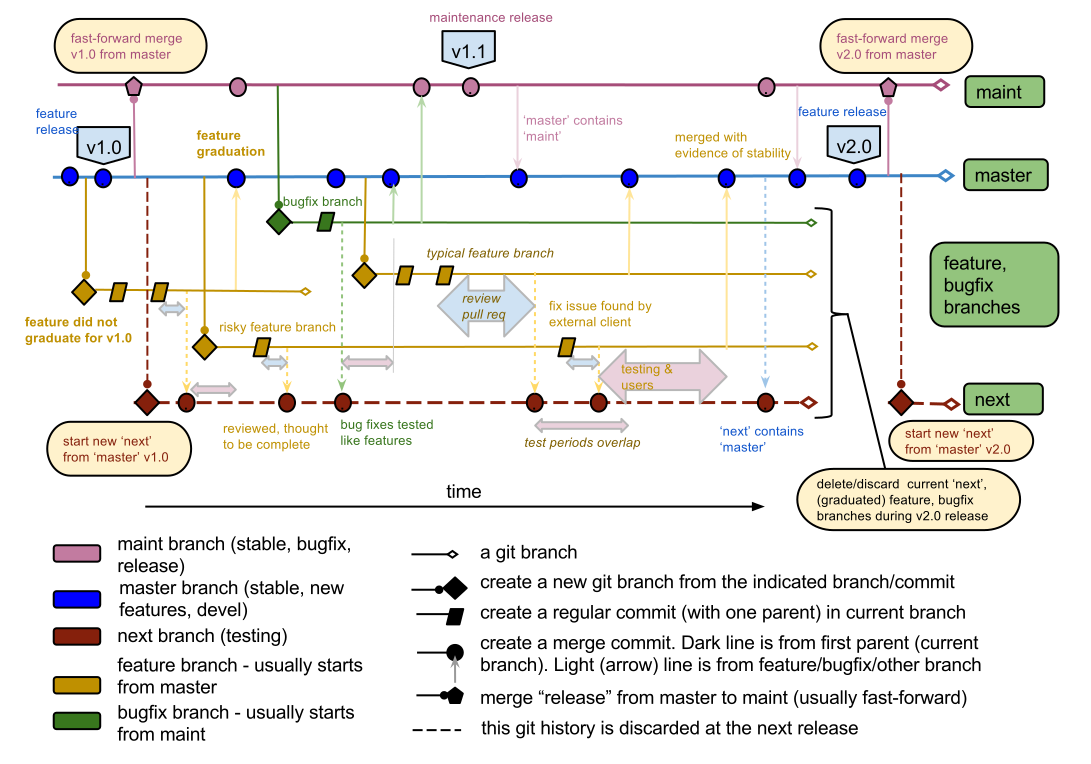
\includegraphics[width=0.85\textwidth]{figures/gitworkflows-satish}
  \end{center}
  \end{block}

  \begin{flushright} \vspace*{-0.5cm}
   \textit{Git is the perl of revision control systems.}
  \end{flushright}
\end{frame}


\begin{frame}{PETSc and Git}
  \begin{center}
    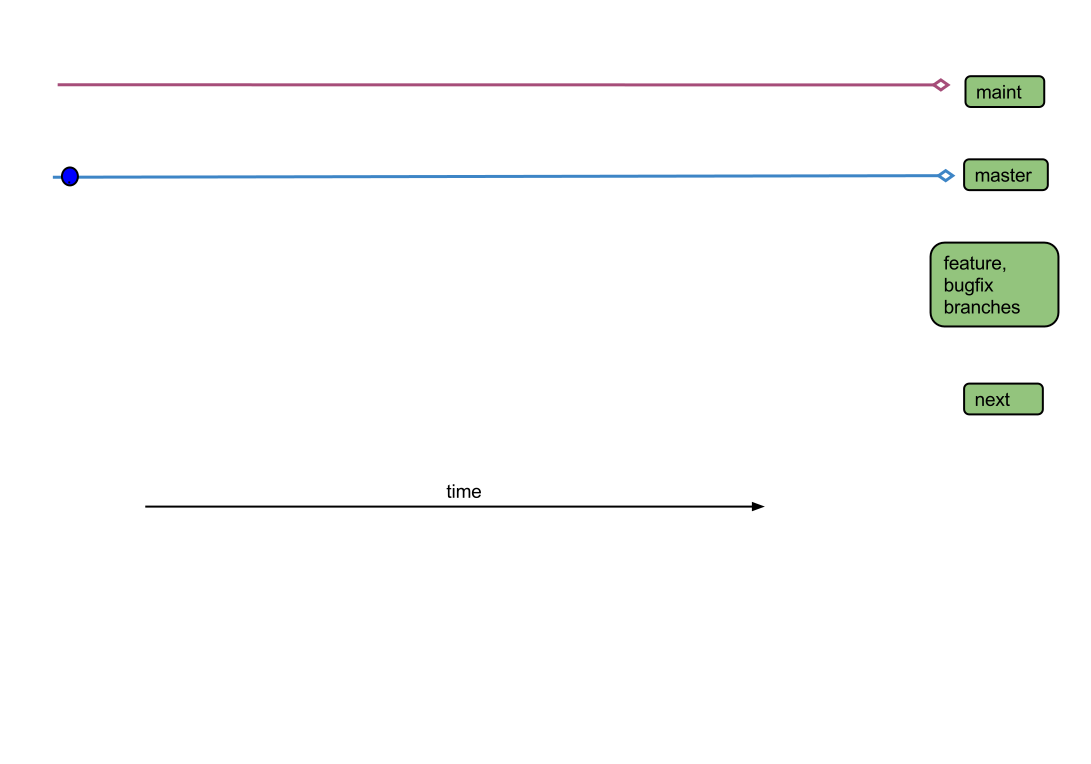
\includegraphics[width=0.99\textwidth]{figures/gitworkflows-45}
  \end{center}
  \begin{flushright} \vspace*{-0.5cm}
   \textit{Oh, yes we all do need that push!}
  \end{flushright}
\end{frame}

\begin{frame}{PETSc and Git}
  \begin{center}
    \includegraphics[width=0.99\textwidth]{figures/gitworkflows-50}
  \end{center}
  \begin{flushright} \vspace*{-0.5cm}
   \textit{It's like we only offer the black belt for people who currently have no belts.}
  \end{flushright}
\end{frame}

\begin{frame}{PETSc and Git}
  \begin{center}
    \includegraphics[width=0.99\textwidth]{figures/gitworkflows-55}
  \end{center}
  \begin{flushright} \vspace*{-0.5cm}
   \textit{If it ain't in email or slashdot then I ain't read it :-)}
  \end{flushright}
\end{frame}

\begin{frame}{PETSc and Git}
  \begin{center}
    \includegraphics[width=0.99\textwidth]{figures/gitworkflows-58}
  \end{center}
  \begin{flushright} \vspace*{-0.5cm}
   \textit{I have now permanently blackholed all email dealing with cygwin.}
  \end{flushright}
\end{frame}

\begin{frame}{PETSc and Git}
  \begin{center}
    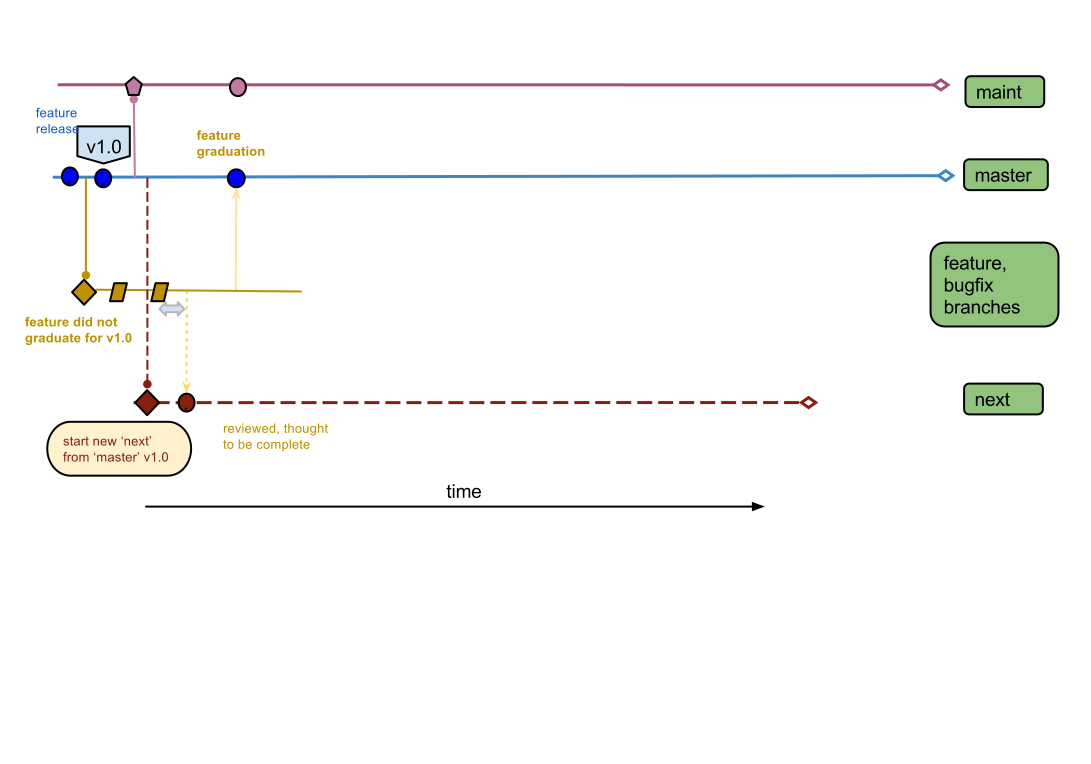
\includegraphics[width=0.99\textwidth]{figures/gitworkflows-60}
  \end{center}
  \begin{flushright} \vspace*{-0.5cm}
   \textit{Peter, Matt gave some bad advice.}
  \end{flushright}
\end{frame}

\begin{frame}{PETSc and Git}
  \begin{center}
    \includegraphics[width=0.99\textwidth]{figures/gitworkflows-65}
  \end{center}
  \begin{flushright} \vspace*{-0.5cm}
   \textit{Satish, please put this in next with the other six million branchs.}
  \end{flushright}
\end{frame}

\begin{frame}{PETSc and Git}
  \begin{center}
    \includegraphics[width=0.99\textwidth]{figures/gitworkflows-70}
  \end{center}
  \begin{flushright} \vspace*{-0.5cm}
   \textit{Don't tell anyone that I put a printf in here}
  \end{flushright}
\end{frame}

\begin{frame}{PETSc and Git}
  \begin{center}
    \includegraphics[width=0.99\textwidth]{figures/gitworkflows-75}
  \end{center}
  \begin{flushright} \vspace*{-0.5cm}
   \textit{I won't call the ICNTL() monstrosity in MUMPS an interface :-)}
  \end{flushright}
\end{frame}

\begin{frame}{PETSc and Git}
  \begin{center}
    \includegraphics[width=0.99\textwidth]{figures/gitworkflows-80}
  \end{center}
  \begin{flushright} \vspace*{-0.5cm}
   \textit{That is all I know about valgrind and it has saved my bacon many times.}
  \end{flushright}
\end{frame}

\begin{frame}{PETSc and Git}
  \begin{center}
    \includegraphics[width=0.99\textwidth]{figures/gitworkflows-85}
  \end{center}
  \begin{flushright} \vspace*{-0.5cm}
   \textit{Stop right here. 99.9\% of the time what you describe should not happen}
  \end{flushright}
\end{frame}

\begin{frame}{PETSc and Git}
  \begin{center}
    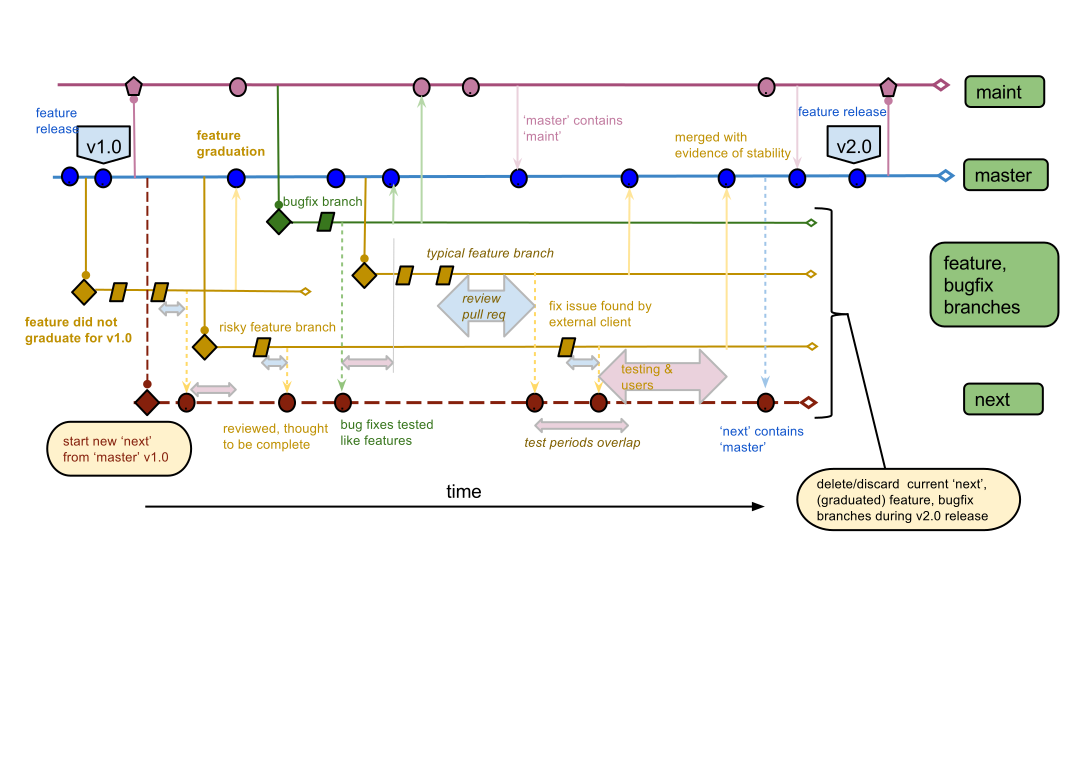
\includegraphics[width=0.99\textwidth]{figures/gitworkflows-90}
  \end{center}
  \begin{flushright} \vspace*{-0.8cm}
   \textit{Git is TeX, what we need is someone to come along\\ and produce LaGit and thus make it usable.}
  \end{flushright}
\end{frame}

\begin{frame}{PETSc and Git}
  \begin{center}
    \includegraphics[width=0.99\textwidth]{figures/gitworkflows-95}
  \end{center}
  \begin{flushright} \vspace*{-1.2cm}
   \textit{Git commands are like irregular verbs in a foreign language: \\
           there’s no all-encompassing logic to them, you just have to memorize \\
           which words you need for each thing you want to express}
  \end{flushright}
\end{frame}





%
% Conclusion and Wrap-Up
%
\section{Conclusions}
\begin{frame}{Conclusions}
 
 \begin{block}{PETSc can Help You}
  \begin{itemize}
   \item solve algebraic and DAE problems in your application area
   \item rapidly develop efficient parallel code, can start from examples
   \item develop new solution methods and data structures
   \item debug and analyze performance
   \item advice on software design, solution algorithms, and performance
   \item \centering \texttt{petsc-\{users,dev,maint\}@mcs.anl.gov}

  \end{itemize}
 \end{block}

 \begin{block}{You can Help PETSc}
  \begin{itemize}
   \item report bugs and inconsistencies, or if you think there is a better way
   \item tell us if the documentation is inconsistent or unclear
   \item consider developing new algebraic methods as plugins, contribute if your idea works
  \end{itemize}
 \end{block}

   \begin{flushright}
   \textit{Thank you!}
  \end{flushright}

\end{frame}

